\chapter{OLD}


\begin{lstlisting}
r: odczytana wartosc      | g: wartosc faktyczna
-----------------------------------------------------
r:_11 g:111 | r:_48 g:148 | r:14_ g:148 | r:_68 g:168
r:_11 g:111 | r:418 g:148 | r:149 g:148 | r:108 g:168
r:_11 g:111 | r:1_8 g:148 | r:1_8 g:168 | r:_0_ g:168
r:_11 g:111 | r:1_8 g:148 | r:108 g:168 | r:_0_ g:168
r:_48 g:148 | r:1_8 g:148 | r:_06 g:168 | r:1_8 g:168
r:_48 g:148 | r:_48 g:148 | r:16_ g:168 | r:1_8 g:168
r:_48 g:148 | r:_48 g:148 | r:14_ g:148 | r:1_8 g:168
r:_48 g:148 | r:_48 g:148 | r:169 g:168 | r:_68 g:168
r:1_8 g:148 | r:149 g:148 | r:108 g:168 | r:_69 g:168
r:418 g:148 | r:149 g:148 | r:166 g:168 | r:_08 g:168
r:108 g:148 | r:149 g:148 | r:16_ g:168 | r:16_ g:168
r:748 g:148 | r:_48 g:148 | r:__8 g:168 | r:1_8 g:168
r:14_ g:148 | r:1_0 g:148 | r:18_ g:168 |
\end{lstlisting}

Na podstawie powyższego wyciągu widać, że poprawienie skuteczności
detektorów kaskadowych powinno wyeliminować znaczną część błędów.
Ogromna większość pomyłek tyczyła się pojedynczych cyfr, kiedy
dwie z~nich - dla pojedycznego, trzycyfrowego numeru - były wykryte
i~odczytane poprawnie.

Dużo mniej błędów odnotowano na drugim etapie odczytu.
Pomyłki przy
klasyfikacji potencjalnych cyfr poprzez dopasowanie wzorców zdarzały 
się co prawda żadziej ale trudniej było im zaradzić.
Na wyciągu poniżej przedstawiono błędy odnotowane na tym etapie.

\begin{lstlisting}
r: 146 g: 148 | r: 166 g: 168 | r: 166 g: 168 | r: 166 g: 168
r: 166 g: 168 | r: 166 g: 168 | r: 166 g: 168
\end{lstlisting}

Pomyłki były w~tym przypadku przy próbie odróżnienia 
cyfry 6 od cyfry 8. Było to ograniczenie, którego 
nie dało się przeskoczyć. Wzorce były bowiem przygotowane dla tego 
konkretnego przypadku i~żadne usprawnienie w~tej kwestii nie było
możliwe. Podobieństwo obu cyfr zostało przedstawione 
na poniższym wyciągu.

\begin{lstlisting}
['6', array([28,  8, 16, 24], dtype=int16), 0.9873822927474976]
['8', array([24,  3, 19, 29], dtype=int16), 0.9856652021408081]
\end{lstlisting}

Na tym etapie zaniechano dalszych prób poprawiania skuteczności 
proponowanego rozwiązania. Pomimo najlepszych starań,
wykorzystując proponowaną metodę nie jest możliwym 
wykonanie skutecznego rozwiązania problemu odczytu 
numeru autobusu przy pomocy wykrywania i~dopasowywania obrazów.
Dalsze prace miały na celu implementację działającego programu na 
urządzeniu mobilnym z~systemem Android.

Dodatkowym utrudnieniem była rozdzielczość i~jakość obrazów rejestrowaych
przy pomocy telefonów. Na rysunku \ref{fig:dist2res} zaprezentowano
stopień degradacji fragmentu obrazu reprezentującego numer
w~zależności od odległości autobusu od obserwatora. 

\begin{figure}[!h]
	\centering
	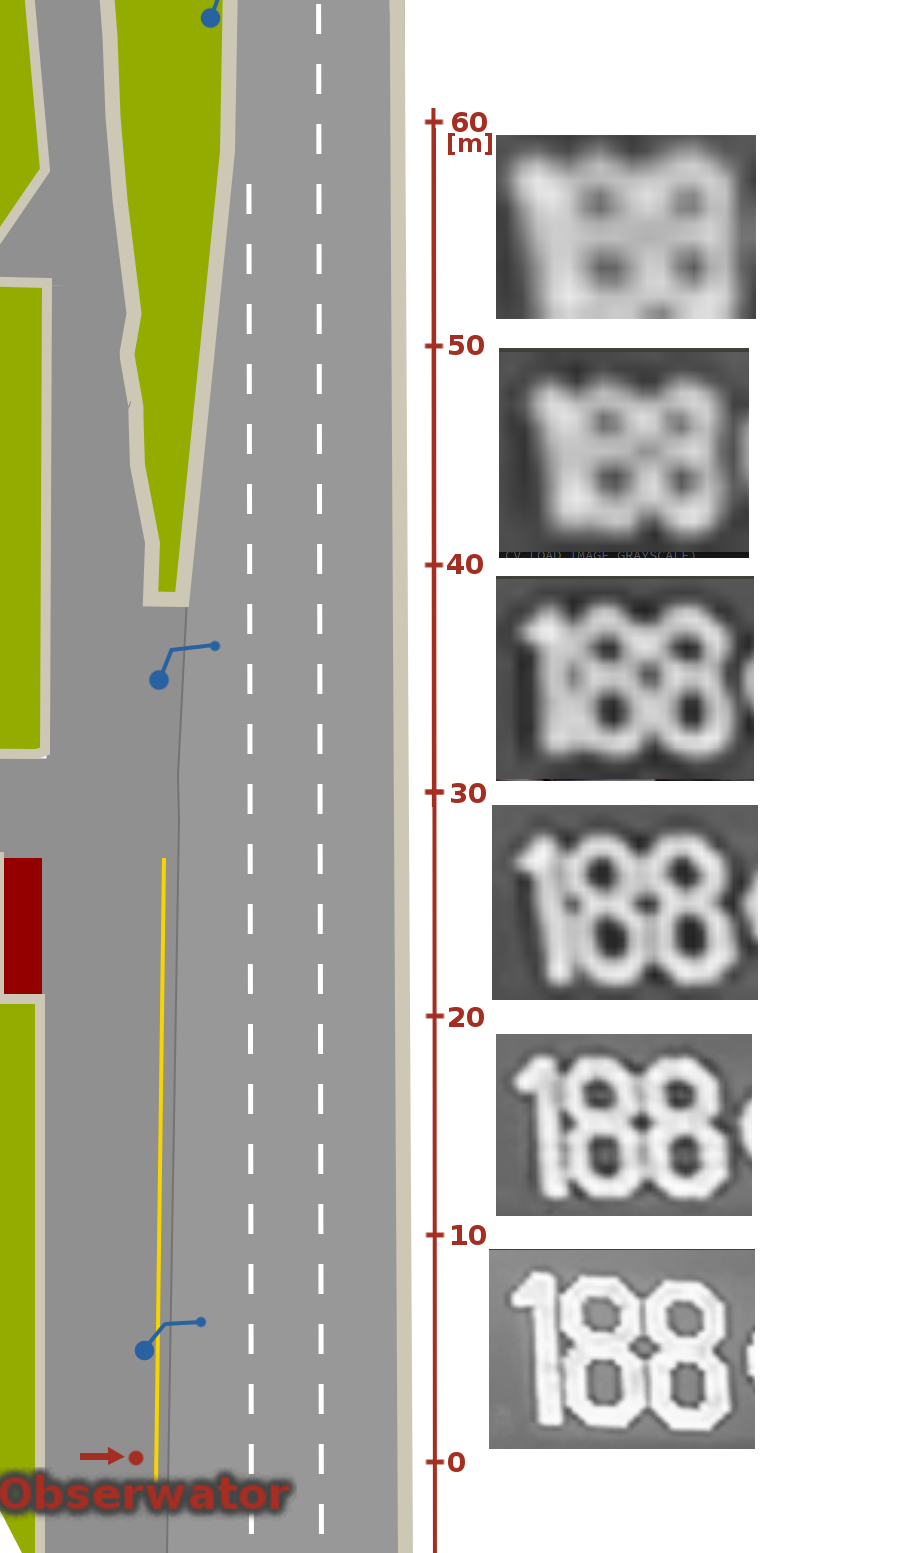
\includegraphics[height=0.9\textwidth]{img/exp_numer_od_odleglosci}
	\caption{Rozdzielczość wykrytego numeru w zależności od odległości}
	\label{fig:dist2res}
\end{figure}

Jakie kolwiek konwencjonalne metody segmentacji były by prawdopodobnie 
możliwe do zastosowani dla odległości frontu mniejszej niż 20 metrów od aparatu.
Jedynym rozwiązaniem jakie mogło by mieć
szanse powodzenia dla większych odległości byłoby wykorzystanie sieci neuronowych. 

\subsubsection{Ostateczna architektura rozwiązania}

Wysokopoziomowa architektura proponowanego rozwiązania była złożona 
z~trzech etapów:
\begin{enumerate}
	\item Odnalezienie frontu autobusu - zawężenie wyszukiwania 
	do kwadratu okalającego front.
	\item Lokalizacja numeru w~obrazie reprezentującym odnaleziony
	front i~przygotowanie odseparowanego numeru jako wejścia
	do funkcji odczytującej tekst.
	\item Odczytanie numeru:
	\begin{itemize}
		\item wyszukanie potencjalnych obszarów reprezentujących
		cyfry,
		\item wyliczenie wartości reprezentującej trafność
		dopasowania cyfry w~wyznaczonym obszarze (template
		matching),
		\item wyznaczanie lokalnych maksimów oraz eliminacja 
		pozostałych teoretycznie błędnych wykryć,
		\item utworzenie ciągu znaków z~wykrytych maksimów,
		zgodnie z~kolejnością występowania w~obrazie -
		wartość odciętych lewego górnego rogu czworokąta
		okalającego.
	\end{itemize}
\end{enumerate}

\begin{figure}[!h]
	\centering
	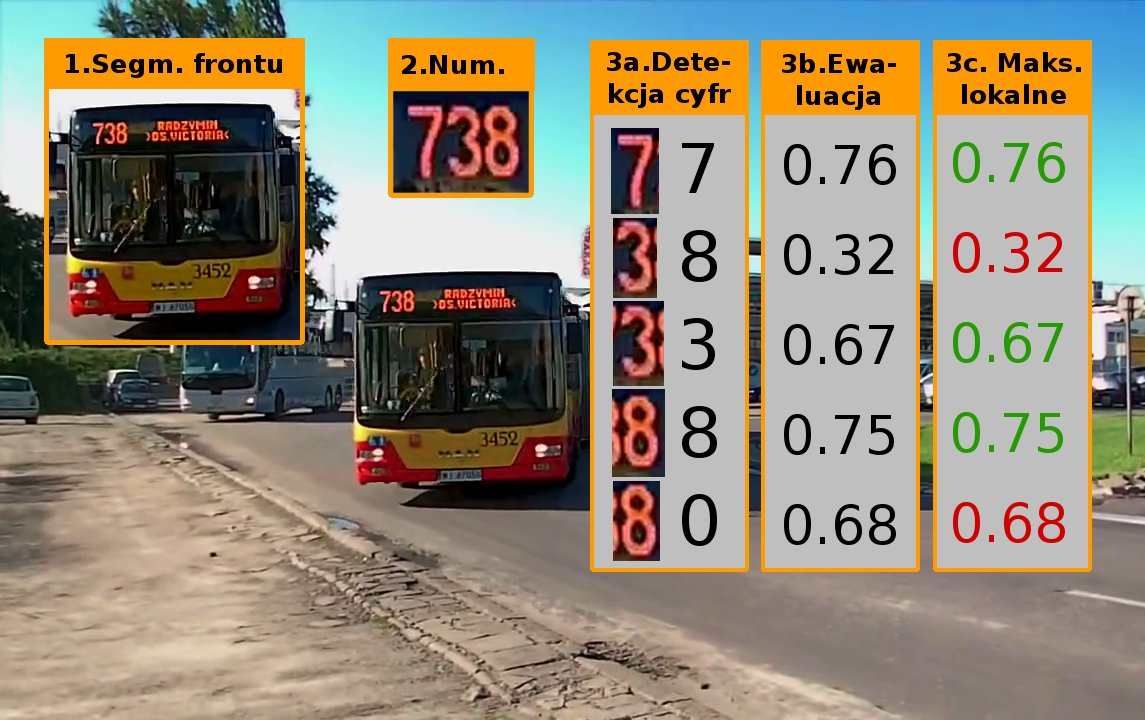
\includegraphics[width=0.9\textwidth]{img/exp_alg_explanation}
	\caption{Graficzne przedstawienie działania algorytmu na przykładzie}
	\label{fig:algexp}
\end{figure}

Rysunek \ref{fig:algexp} przedstawia przykładowy przebieg kaskady. 
Na początku wykrywany i~lokalizowany był front autobusu.
Następnie wyłuskiwany był fragment zawierający wyłącznie numer linii.
Ostatecznie następował odczyt. Na zadanym fragmencie uruchamianych było
10 detektorów dla poszczególnych cyfr. Obrazy wynikowe - potencjalnie
cyfry - przeskalowywano do zadanej wysokości z~zachowaniem proporcji.
Dla tak przygotowanych fragmentów uruchamiano narzędzie wiliczające
trafność dopasowania. Wykorzystano w~tym celu
mechanizm templateMatching. W~przypadku
gdy na przykład detektor trójek
wykryłby ósemkę (lub na odwrót), powinna dostać ona niską
ocenę przy dopasowaniu tychże trójek. Ostatecznie mając
zbiór czworokątów okalających z~przypisanymi do nich wartościami
wybierane były te o~najwyższych wynikach. W~określaniu ważna była też
odległość między cyframi. Gdyby nie wprowadzono tego kryterium
w~prezentowanym przykładzie wynik składał by się z~cyfr 7, 8 oraz 0.
Które to zero zostało wyeliminowane ze względu na zbyt bliskie położenie
względem wykrytej cyfry 8 z~wyższym wynikiem.

Na rysunku \ref{fig:finaltest} zaprezentowano jeden z~ostanich 
testów podglądowych przed implementacją programu na telefonie.

\begin{figure}[!h]
	\centering
	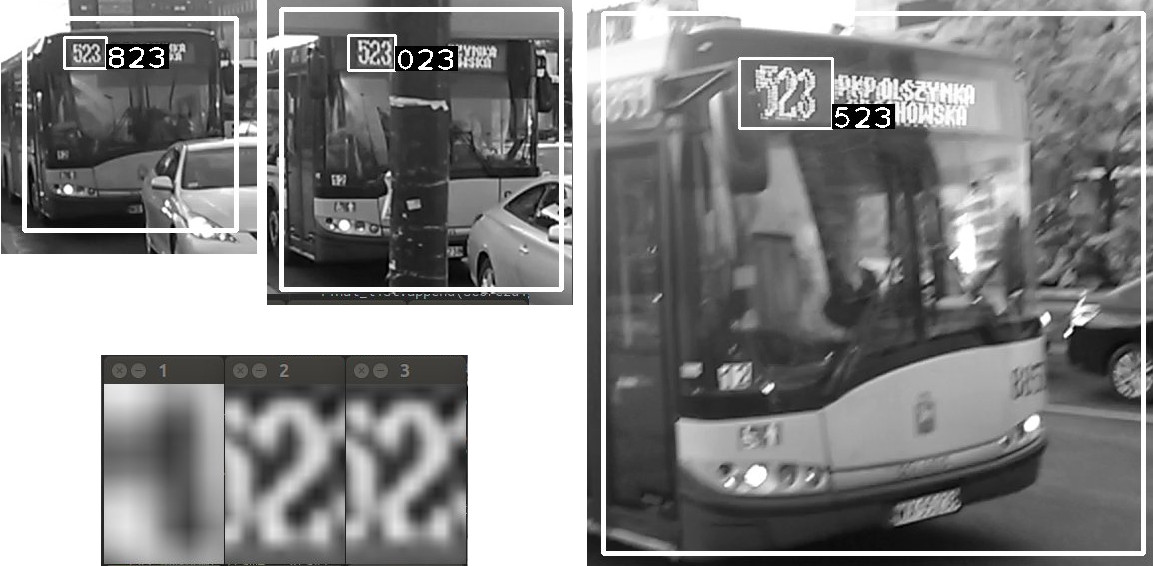
\includegraphics[width=0.9\textwidth]{img/exp_final_test}
	\caption{Ostatni test przed implementacją na telefonie}
	\label{fig:finaltest}
\end{figure}

W~lewym dolnym rogu rysunku można zaobserwować okienka prezentujące
wyniki działania detektorów do wyszukiwania cyfr. Jak nie trudno
zgadnąć były one najmniej precyzyjnym elementem całego systemu.
W~ramach dalszych prac niezbędnym byłoby usprawnienie
skuteczności detekcji, tak aby detektory wykrywały jak 
najwięcej poprawnych (i niepoprawnych) fragmentów
reprezentujących cyfry. Do rozwiązania jest też problem
bliskiej odległości - dużego podobieństwa cyfr - kiedy to
metoda template matching nie jest w~stanie rozróżnić cyfr o~podobnym
kształcie, np. 9,8,6.

\subsection{Testy całego algorytmu}

Po przygotowaniu zbioru 1903 obrazów zawierających fronty autobusów
z~wyświetlaczem led przystąpiono do automatycznej weryfikacji 
skuteczności pierwotnego algorytmu zaimplementowanego na urządzeniu
w~ramach pierwszej iteracji.
Pliki z~frontami autobusów posiadały numer linii w~nawie pliki. 
Na tej podstawie automat weryfikował wynik otrzymany od narzędzia
poddawanego testom.


\begin{table}[!h]
	\centering
	\begin{tabular}{c|c|c}
		Wykryte fronty  & Wykryte numeru & Poprawne odczyty \\ \hline
		1119 & 1016 & 551
	\end{tabular}
	\caption{Ilość wykrytych frontów, numerów i ogólnych poprawnych 
		odczytów pierwszej wersji algorytmu}
	\label{tab:first_version_results}
\end{table}

Wyniki zamieszczone w~tabeli \ref{tab:first_version_results}
reprezentują ilość poprawnych odczytów na próbce testowej
liczącej 1903 fronty autobusów. Końcowa skuteczność
pierwszej wersji algorytmu jest więc na poziomie 29\%.

Wykorzystując parametry detektora frontów uzyskane w~drugiej
iteracji uzyskano znacznie lepsze wyniki zaprezentowane w~tabeli
\ref{tab:second_version_results}.

\begin{table}[!h]
	\centering
	\begin{tabular}{c|c|c}
		Wykryte fronty  & Wykryte numeru & Poprawne odczyty \\ \hline
		1820 & 1609 & 845
	\end{tabular}
	\caption{Ilość wykrytych frontów, numerów i ogólnych poprawnych 
		odczytów drugiej wersji algorytmu (detektor frontów)}
	\label{tab:second_version_results}
\end{table}

Ogólna skuteczność wzrosła do 44\%. Jest to nadal kiepski wynik.
Co jest tu jednak niezwykle ważne to to, że 
poprzez poprawę jednego elementu
poprawiono ogólną skuteczność o~15\%.

Poprzez podmianę detektora numerów, na ten wytrenowany 
podczas drugiej iteracji otrzymano rezultaty widoczne
w~tabeli \ref{tab:upset_second_version_number_detector}.

\begin{table}[!h]
	\centering
	\begin{tabular}{c|c|c}
		Wykryte fronty  & Wykryte numeru & Poprawne odczyty \\ \hline
		1820 & 1517 & 764 
	\end{tabular}
	\caption{Ilość wykrytych frontów, numerów i ogólnych poprawnych 
		odczytów drugiej wersji algorytmu (detektor frontów)}
	\label{tab:upset_second_version_number_detector}
\end{table}

Pomimo wysokiej skuteczności w~teście syntetycznym
detektor numerów z~drugiej iteracji miał gorszą skuteczność
niż pierwszy prototyp. Otrzymano też dużo gorszy wynik
ogólny, bo skuteczność całego rozwiązania spadła do
40\%.

Ostatni przykład, czyli gorszy wynik dla teoretycznie 
lepszego detektora świetnie pokazuje jak ważny jest zbiór
danych, jego jakość i~co najważniejsze liczność. 
W~celu rzetelnego przebadania skuteczności zbiór danych 
rzędu kilku tysięcy to zbyt mało. Szczególnie gdy część 
z~tych danych służyła też jako zbiór uczący.
W~przypadku tak skomplikowanych obiektów wymagane są 
dane liczone w~dziesiątkach o~ile nie setkach tysięcy.
Przykładem może być publiczny zbiór danych SVHN.

Na tym etapie wstrzymano się od dalszej optymalizacji. 
Proponowane rozwiązanie wymaga jeszcze dużo pracy nad 
doskonaleniem poszczególnych jego elementów.
Jest jednak wielce prawdopodobne, że po dopracowaniu 
wszystkich kroków skuteczność będzie więcej niż zadowalająca.